            The proof of the following claim is straightforward, and is
        included for the sake of completeness.  Let
        $\epsA = \min( \eps, \delta^2)$. Construct, in
        $\Of(\epsA^{-1} n \log n)$ time, any standard $(1+\epsA)$-spanner
        $\G$ for $\PS$ using $\Of( \epsA^{-1} n)$ edges (e.g.,
        \cite{ams-dagss-99}).
        
        So, consider any body $\body \in \FF$, and any two points
        $\pa, \pb \in \PS \cap \body'$, where
        $\body'=\shrinkDY{\body}{\delta}$, let $\ell = \dY{\pa}{\pb}$, let
        $\pi$ be the shortest path between $\pa$ and $\pb$ in $\G$, and
        let $\Elp$ be the locus of all points $\pc$, such that
        $\dY{\pa}{\pc} + \dY{\pc}{\pb} \leq (1+\epsA) \ell$. The region
        $\Elp$ is an ellipse that contains $\pi$. The furthest point from
        the segment $\pa\pb$ in this ellipse is realized by the co-vertex
        of the ellipse. Formally, it is one of the two intersection points
        of the boundary of the ellipse with the line orthogonal to
        $\pa \pb$ that passes through the middle point $\cen$ of this
        segment, see \figref{ellipse}. Let $\pz$ be one of these points.
        
        \begin{figure}[h]
                \centerline{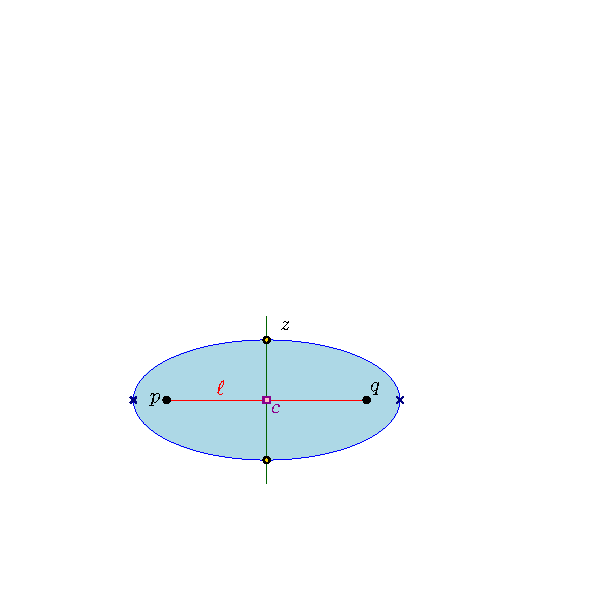
\includegraphics{../figs/ellipse}}
                \caption{An illustration of the settings in the proof of
                        \lemref{w:l:s:regions} with $\Elp$ shown in blue.}
                \figlab{ellipse}
        \end{figure}
        
        We have that
        \begin{math}
                \dY{\pa}{\pz} = (1+\epsA)\ell/2.
        \end{math}
        Setting $h = \dY{\pz}{\cen}$, we have that
        \begin{equation*}
                h%
                =%
                \sqrt{\dY{\pa}{\pz}^2 - \dY{\pa}{\cen}^2 }
                =%
                \frac{\ell}{2} \sqrt{(1+\epsA)^2 - 1}
                =%
                \frac{\sqrt{\epsA (2+\epsA)}}{2} \ell%
                \leq
                \sqrt{\epsA} \ell
                \leq
                \sqrt{\epsA}\cdot \diameterX{\body}.
        \end{equation*}
        as $\ell \leq \diameterX{\body'} \leq \diameterX{\body}$.
        
        For any point $\px \in \body'$, we have that
        $\dsY{\px}{\Re^2 \setminus \body} \geq \delta \cdot
        \diamX{\body}$.  As such, to ensure that
        $\pi \subseteq \Elp \subseteq \body$, we need that
        \begin{math}
                \delta \cdot \diamX{\body} \geq h,
        \end{math}
        which holds if
        \begin{math}
                \delta \cdot \diamX{\body} \geq \sqrt{\epsA} \cdot
                \diameterX{\body}.
        \end{math}
        This in turn holds if $\epsA \leq \delta^2$. Namely, we have
        the desired properties if $\epsA = \min( \eps, \delta^2)$.
